% Credits are indicated where needed. The general idea is based on a template by Vel (vel@LaTeXTemplates.com) and Frits Wenneker.

\documentclass[11pt, a4paper]{article} % General settings in the beginning (defines the document class of your paper)
% 11pt = is the font size
% A4 is the paper size
% “article” is your document class

%----------------------------------------------------------------------------------------
%	Packages
%----------------------------------------------------------------------------------------

% Necessary
\usepackage[german,english]{babel} % English and German language 
\usepackage{hyperref} % URL
\usepackage{subfig} %two figure
\usepackage{listings} % Insert code
\usepackage{float} % figure at the correct position
\usepackage{lipsum}
\usepackage{mwe}
\usepackage{booktabs} % Horizontal rules in tables 
% For generating tables, use “LaTeX” online generator (https://www.tablesgenerator.com)
\usepackage{comment} % Necessary to comment several paragraphs at once
\usepackage[utf8]{inputenc} % Required for international characters
\usepackage[T1]{fontenc} % Required for output font encoding for international characters

% Might be helpful
\usepackage{amsmath,amsfonts,amsthm} % Math packages which might be useful for equations
\usepackage{tikz} % For tikz figures (to draw arrow diagrams, see a guide how to use them)
\usepackage{tikz-cd}
\usetikzlibrary{positioning,arrows} % Adding libraries for arrows
\usetikzlibrary{decorations.pathreplacing} % Adding libraries for decorations and paths
\usepackage{tikzsymbols} % For amazing symbols ;) https://mirror.hmc.edu/ctan/graphics/pgf/contrib/tikzsymbols/tikzsymbols.pdf 
\usepackage{blindtext} % To add some blind text in your paper


%---------------------------------------------------------------------------------
% Additional settings
%---------------------------------------------------------------------------------

%---------------------------------------------------------------------------------
% Define your margins
\usepackage{geometry} % Necessary package for defining margins

\geometry{
	top=2cm, % Defines top margin
	bottom=2cm, % Defines bottom margin
	left=2.2cm, % Defines left margin
	right=2.2cm, % Defines right margin
	includehead, % Includes space for a header
	%includefoot, % Includes space for a footer
	%showframe, % Uncomment if you want to show how it looks on the page 
}

\setlength{\parindent}{15pt} % Adjust to set you indent globally 

%---------------------------------------------------------------------------------
% Define your spacing
\usepackage{setspace} % Required for spacing
% Two options:
\linespread{1.5}
%\onehalfspacing % one-half-spacing linespread

%----------------------------------------------------------------------------------------
% Define your fonts
\usepackage[T1]{fontenc} % Output font encoding for international characters
\usepackage[utf8]{inputenc} % Required for inputting international characters

\usepackage{XCharter} % Use the XCharter font


%---------------------------------------------------------------------------------
% Define your headers and footers

\usepackage{fancyhdr} % Package is needed to define header and footer
\pagestyle{fancy} % Allows you to customize the headers and footers

%\renewcommand{\sectionmark}[1]{\markboth{#1}{}} % Removes the section number from the header when \leftmark is used

% Headers
\lhead{} % Define left header
\chead{\textit{}} % Define center header - e.g. add your paper title
\rhead{} % Define right header

% Footers
\lfoot{} % Define left footer
\cfoot{\footnotesize \thepage} % Define center footer
\rfoot{ } % Define right footer

%---------------------------------------------------------------------------------
%	Add information on bibliography
\usepackage{natbib} % Use natbib for citing
\usepackage{har2nat} % Allows to use harvard package with natbib https://mirror.reismil.ch/CTAN/macros/latex/contrib/har2nat/har2nat.pdf

% For citing with natbib, you may want to use this reference sheet: 
% http://merkel.texture.rocks/Latex/natbib.php

%---------------------------------------------------------------------------------
% Add field for signature (Reference: https://tex.stackexchange.com/questions/35942/how-to-create-a-signature-date-page)
\newcommand{\signature}[2][5cm]{%
  \begin{tabular}{@{}p{#1}@{}}
    #2 \\[2\normalbaselineskip] \hrule \\[0pt]
    {\small \textit{Signature}} \\[2\normalbaselineskip] \hrule \\[0pt]
    {\small \textit{Place, Date}}
  \end{tabular}
}
%---------------------------------------------------------------------------------
%	General information
%---------------------------------------------------------------------------------
\title{Deep Learning HW3 Report} % Adds your title
%\author
%{
%    \name{Alfons Hwu} % Add your first and last name
%    %\thanks{} % Adds a footnote to your title
%    \\
%    \institution{0416324, Dept of Computer Science NCTU} % Adds your institution
%}



%---------------------------------------------------------------------------------
%	Define what’s in your document
%---------------------------------------------------------------------------------
\begin{document}


% If you want a cover page, uncomment "%---------------------------------------------------------------------------------
% Cover page
%---------------------------------------------------------------------------------

% Here are more templates for other cover pages: https://www.latextemplates.com/cat/title-pages

% This example is based on this cover page example: https://www.latextemplates.com/template/academic-title-page

\begin{titlepage} % Starts new environment where the page number is not displayed and the count starts at 1 for the next page

%------------------------------------------------
%	Institutional information
%------------------------------------------------
	
\begin{minipage}{0.4\textwidth} % Begins new environment (like a text box)
    \begin{flushleft} % Sets environment on the left side of the paper
    \large
    National Chiao Tung University\\ % Add your institution
    Spring 2019 \\ % Add term
    Deep Learning \\ % Add course title
    Instructor: Jen-Tsung Chien\\ % Add instructor/supervisor name 
    \end{flushleft}
\end{minipage}
	
\vspace*{2in} % Adds some space in-between
	
\center % Centre everything on the page

%------------------------------------------------
%	Main part
%------------------------------------------------
	
{\huge\bfseries Deep Learning HW2 Report}\\[0.4cm] % Add your paper title {\large\today}\\[0.4cm] % Add date (current day)
Alfons Hwu \\ % Add your name
Student ID: 0416324\\
\vfill % Adds additional space

%------------------------------------------------
%	General information about the author
%------------------------------------------------

\vfill % Adds additional space

alfons.cs04@g2.nctu.edu.tw \\ % Add your contact info
Dept of Computer Science \\ % Add info about your program
Writing with \LaTeX  on Overleaf

\vfill % Adds additional space

%------------------------------------------------
%	Word count
%------------------------------------------------

\vfill % Adds additional space
	
\end{titlepage}" and uncomment "\begin{comment}" and "\end{comment}" to comment the following lines
%---------------------------------------------------------------------------------
% Cover page
%---------------------------------------------------------------------------------

% Here are more templates for other cover pages: https://www.latextemplates.com/cat/title-pages

% This example is based on this cover page example: https://www.latextemplates.com/template/academic-title-page

\begin{titlepage} % Starts new environment where the page number is not displayed and the count starts at 1 for the next page

%------------------------------------------------
%	Institutional information
%------------------------------------------------
	
\begin{minipage}{0.4\textwidth} % Begins new environment (like a text box)
    \begin{flushleft} % Sets environment on the left side of the paper
    \large
    National Chiao Tung University\\ % Add your institution
    Spring 2019 \\ % Add term
    Deep Learning \\ % Add course title
    Instructor: Jen-Tsung Chien\\ % Add instructor/supervisor name 
    \end{flushleft}
\end{minipage}
	
\vspace*{2in} % Adds some space in-between
	
\center % Centre everything on the page

%------------------------------------------------
%	Main part
%------------------------------------------------
	
{\huge\bfseries Deep Learning HW2 Report}\\[0.4cm] % Add your paper title {\large\today}\\[0.4cm] % Add date (current day)
Alfons Hwu \\ % Add your name
Student ID: 0416324\\
\vfill % Adds additional space

%------------------------------------------------
%	General information about the author
%------------------------------------------------

\vfill % Adds additional space

alfons.cs04@g2.nctu.edu.tw \\ % Add your contact info
Dept of Computer Science \\ % Add info about your program
Writing with \LaTeX  on Overleaf

\vfill % Adds additional space

%------------------------------------------------
%	Word count
%------------------------------------------------

\vfill % Adds additional space
	
\end{titlepage}

\date{June 5, 2019}
\begin{comment}
\end{comment}
\maketitle{} %Print your title, author name and date; comment if you want a cover page 

%----------------------------------------------------------------------------------------
% Introduction
%----------------------------------------------------------------------------------------
\setcounter{page}{1} % Sets counter of page to 1

\section{Self-designed VAE for image reconstruction and generating(unsupervised learning)} % Add a section title
\subsection{Preprocessing the images} % Section check OK 20190502
In the preprocessing part, I merely resize the image to 64 x 64 and without normalization. 
\\ If normalization is used, the reconstructed / randomly generated image will look very dark and black.
\\ CNN is used in this problem since it \textbf{fits better for image processing} while DNN falls short in this part because it processes 3 color channels at the same time, causing the result image somehow looked grey(The value of R G B are similar).
\\ The CNN layers are used in the feature extraction and reconstruction part as the following code shows.
\begin{lstlisting}[language = python]
def __init__(self, image_channels = 3, h_dim = 1024, z_dim = 32):
        super(VAE, self).__init__()
        self.encoder = nn.Sequential(
            nn.Conv2d(image_channels, 32, kernel_size = 4, stride = 2),
            nn.ReLU(),
            nn.Conv2d(32, 64, kernel_size = 4, stride = 2),
            nn.ReLU(),
            nn.Conv2d(64, 128, kernel_size = 4, stride = 2),
            nn.ReLU(),
            nn.Conv2d(128, 256, kernel_size = 4, stride = 2),
            nn.ReLU(),
            flatten()
        )
        self.fc1 = nn.Linear(h_dim, z_dim)
        self.fc2 = nn.Linear(h_dim, z_dim)
        self.fc3 = nn.Linear(z_dim, h_dim)
        # The code of decoder part is just deconvolution, i.e. nn.ConvTranspose2d with reverse order and I/O dimension
        )
\end{lstlisting}
\\ Between the feature extraction and image reconstruction lies the reparameterization part, that is by multiplying $\sigma$ and shifting $\mu$, making $N~(0, 1)$ to approximate $N~(\mu, \sigma^2)$
\begin{figure}[H]
  \centering
  \subfloat[VAE ovaerall architecture]{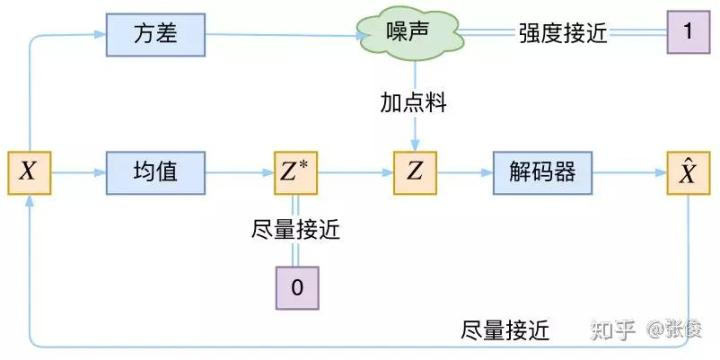
\includegraphics[scale = 0.3]{HW3/vae/vae_arch.jpg}\label{fig:f1}}
  \hfill
  \subfloat[Reparameterization to approximate $N~(0, 1)$]{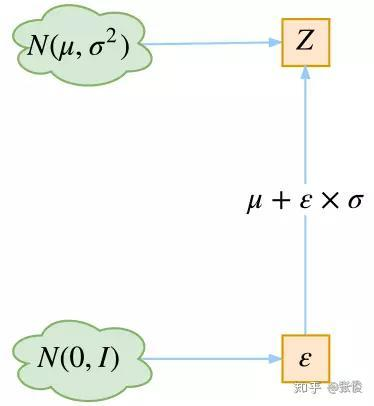
\includegraphics[scale = 0.3]{HW3/vae/reparam.jpg}\label{fig:f2}}
  \hfill
  \subfloat[Mathematical explanation]{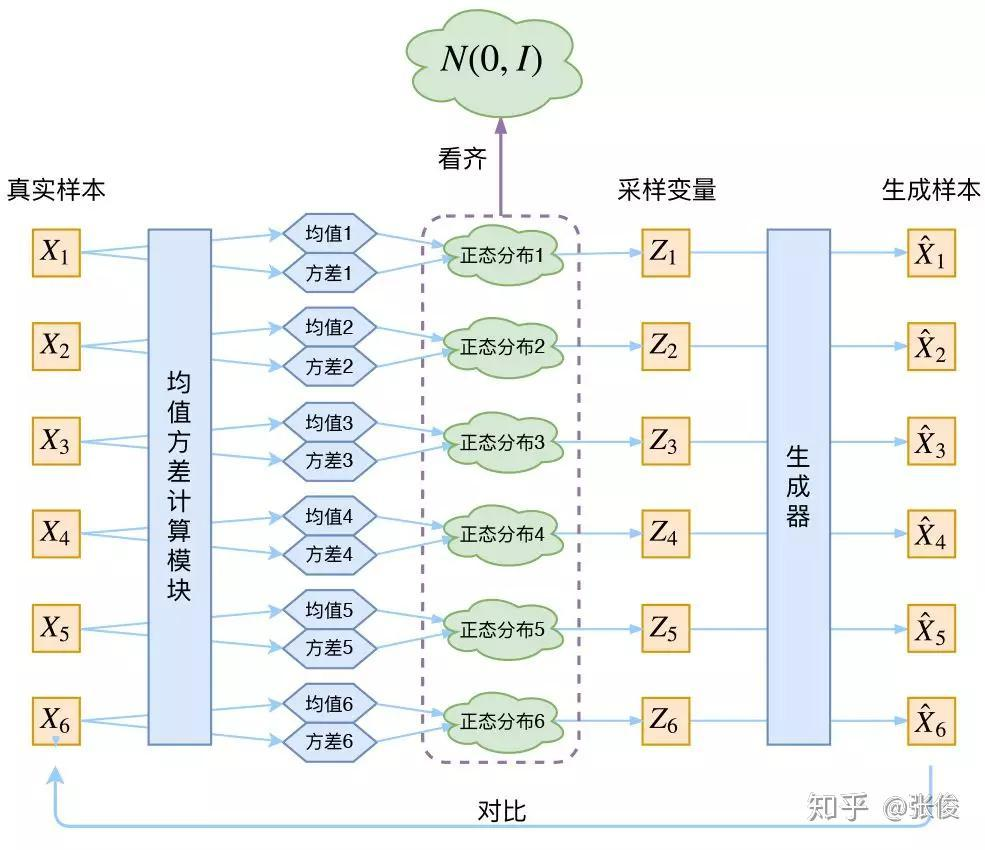
\includegraphics[scale = 0.2]{HW3/vae/vae_idea.jpg}\label{fig:f2}}
  \hfill
  \caption{VAE explanation}
\end{figure}
\\ \small{Image source credit to \url{https://zhuanlan.zhihu.com/p/34998569}}

\subsection{Learning curve and reconstructed images}
\begin{figure}[H]
    \centering
    \subfloat[Learning curve]{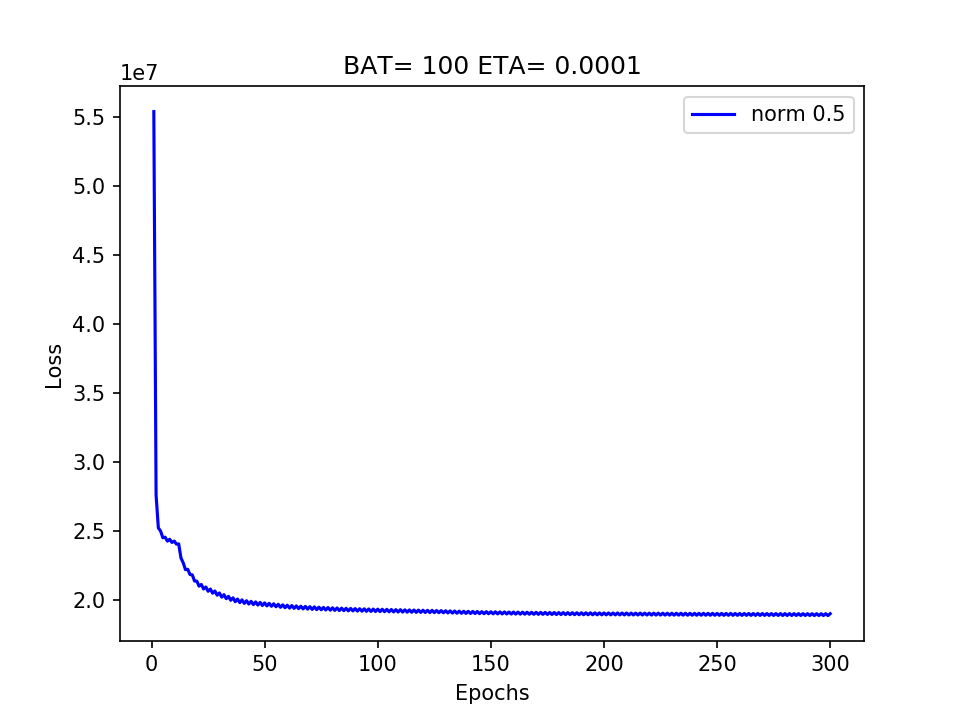
\includegraphics[scale = 0.9]{HW3/vae_result/lc.png}\label{fig:f1}}
    \hfill
    \subfloat[Reconstructed image]{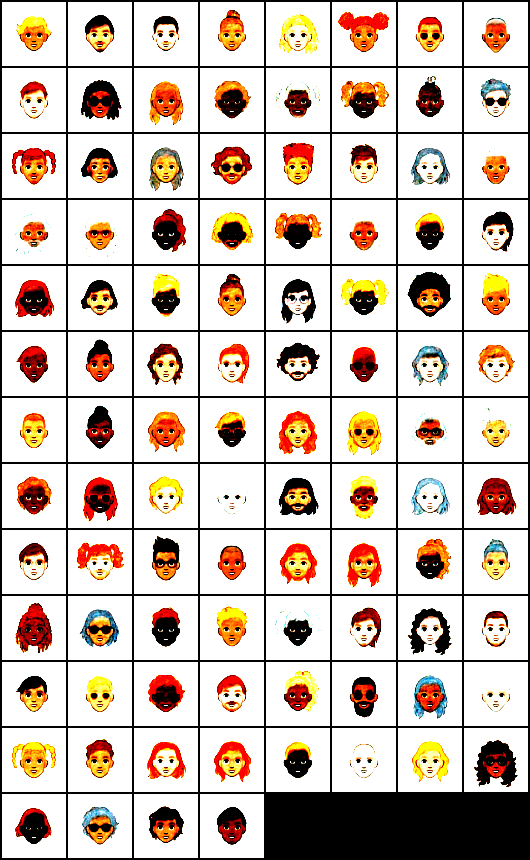
\includegraphics[scale = 0.3]{HW3/vae_result/re.png}\label{fig:f2}}
    \hfill
    \subfloat[Ground truth]{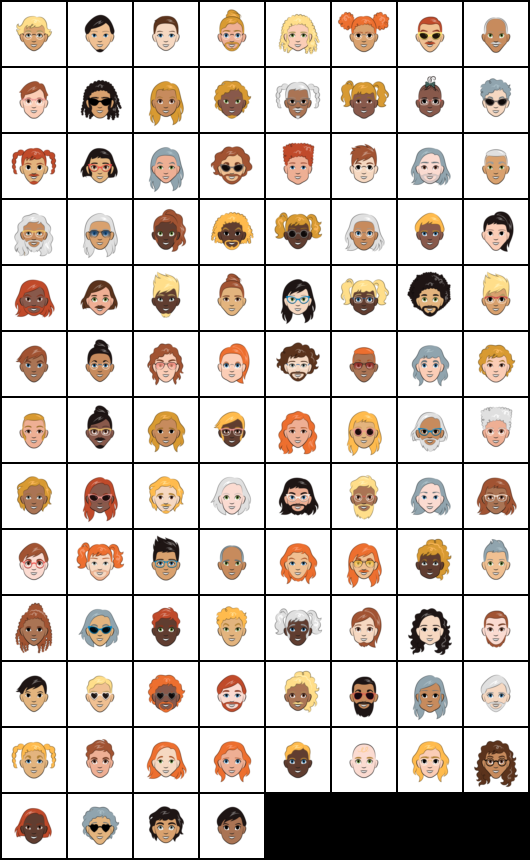
\includegraphics[scale = 0.3]{HW3/vae_result/gt.png}\label{fig:f2}}
    \hfill
    \caption{VAE result evaluation}
\end{figure}
\\ \textbf{KL annealing} is used in this model to improve learning different characteristics from different faces, since without it, KL Divergence and Loss will be quite small, and with small error value, NN will be hard to implement self-learning, causing the whole reconstructed image to be all the same (bulrry, averaging all the characteristics of all images).
\\ KL annealing reference to \url{http://www.sohu.com/a/216987798_297288}
\begin{figure}[H]
    \centering
    \subfloat[Without KL annealing]{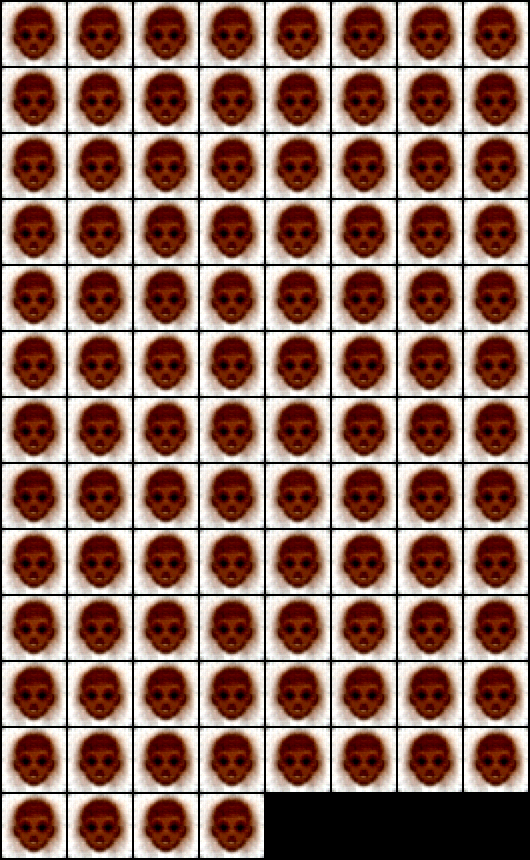
\includegraphics[scale = 0.4]{HW3/vae_result/re_no.png}\label{fig:f1}}
    \hfill
    \subfloat[With KL annealing]{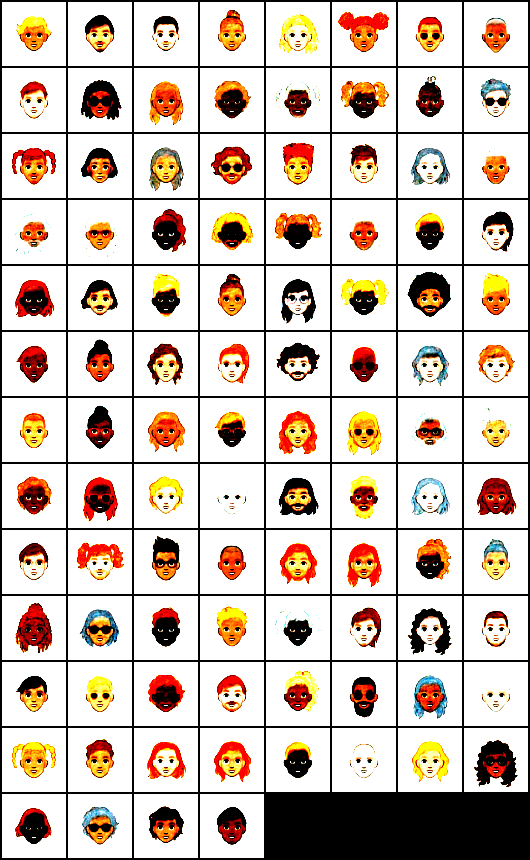
\includegraphics[scale = 0.4]{HW3/vae_result/re.png}\label{fig:f2}}
    \hfill
    \caption{Comparison}
\end{figure}

\subsection{Randomly generated images}
\begin{figure}[H]
    \centering
    \subfloat[Generated 1]{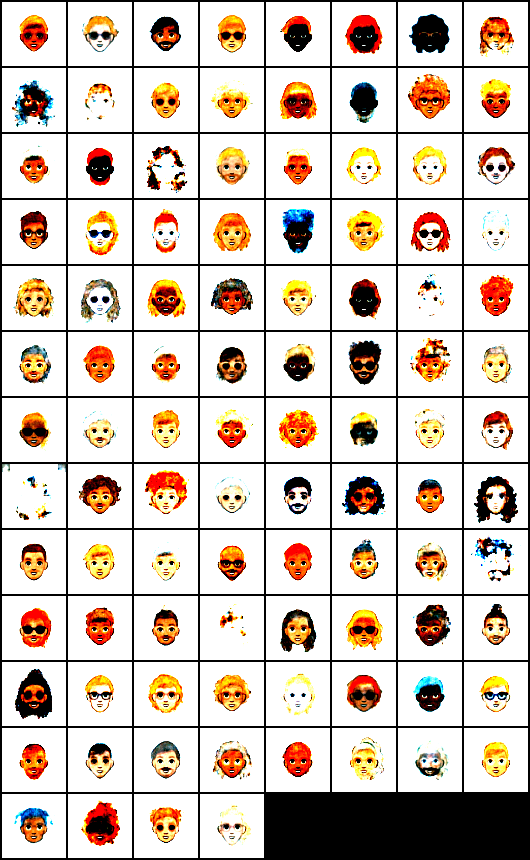
\includegraphics[scale = 0.4]{HW3/vae_result/gen_1.png}\label{fig:f1}}
    \hfill
    \subfloat[Generated 2]{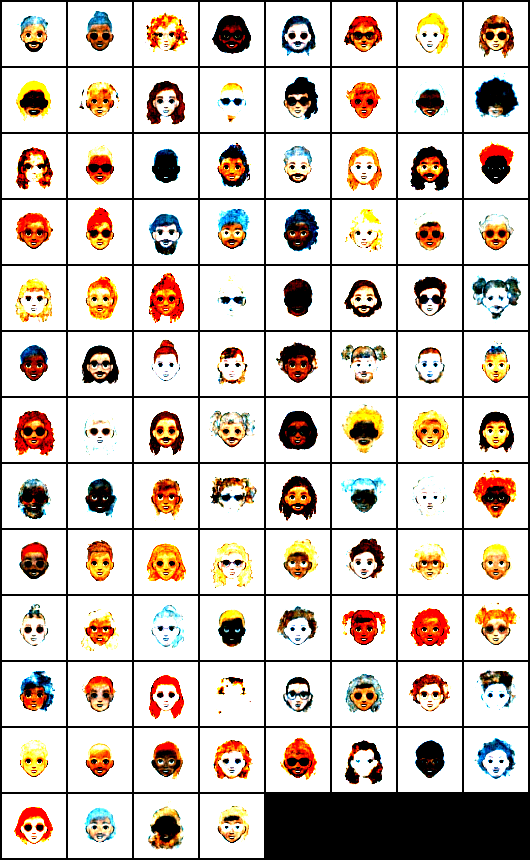
\includegraphics[scale = 0.4]{HW3/vae_result/gen_2.png}\label{fig:f2}}
    \hfill
    \caption{Generated images}
\end{figure}
\section{Self-designed CGAN for style transformation(unsupervised learning)}
\subsection{Loss curves of discriminator and generator}
\begin{figure}[H]
    \centering
    \subfloat[Loss curve of discriminator]{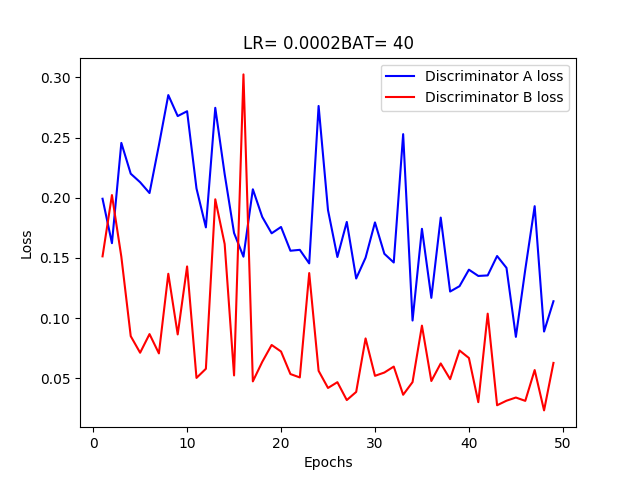
\includegraphics[scale = 0.5]{HW3/cgan_result/dis.png}\label{fig:f1}}
    \hfill
    \subfloat[Loss curve of generator]{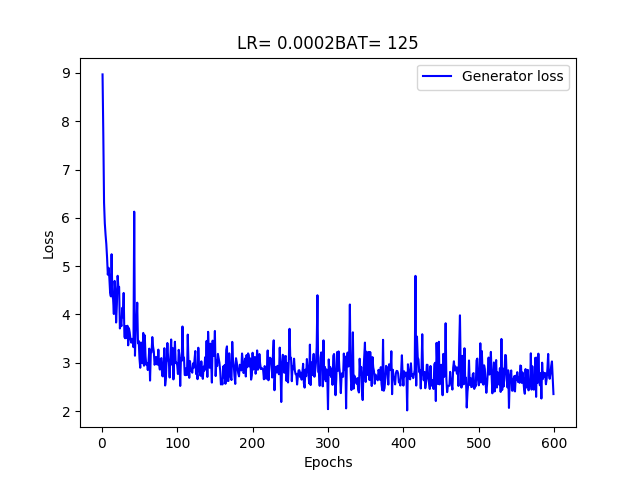
\includegraphics[scale = 0.5]{HW3/cgan_result/gen.png}\label{fig:f2}}
    \hfill
    \caption{Loss curves}
\end{figure}

\subsection{Results of style transferred images}
\begin{figure}[H]
    \centering
    \subfloat[Real cartoon 1]{
\includegraphics[scale = 1.0]{HW3/transfer/rc_1.png}\label{fig:f1}}
    \hfill
    \subfloat[Real cartoon 2]{
\includegraphics[scale = 1.0]{HW3/transfer/rc_2.png}\label{fig:f2}}
    \hfill
    \subfloat[Fake anime 1(From real cartoon 1)]{
\includegraphics[scale = 1.0]{HW3/transfer/fa_1.png}\label{fig:f2}}
    \hfill
    \subfloat[Fake anime 2(From real cartoon 2)]{
\includegraphics[scale = 1.0]{HW3/transfer/fa_2.png}\label{fig:f2}}
    \hfill
    \caption{Transfer from cartoon(real cartoon in ground truth) to anime(fake anime generated by GAN)}
\end{figure}

\begin{figure}[H]
    \centering
    \subfloat[Real anime 1]{
\includegraphics[scale = 1.0]{HW3/transfer/ra_1.png}\label{fig:f1}}
    \hfill
    \subfloat[Real anime 2]{
\includegraphics[scale = 1.0]{HW3/transfer/ra_2.png}\label{fig:f2}}
    \hfill
    \subfloat[Fake cartoon 1(From real anime 1)]{
\includegraphics[scale = 1.0]{HW3/transfer/fc_1.png}\label{fig:f2}}
    \hfill
    \subfloat[Fake cartoon 2(From real anime 2)]{
\includegraphics[scale = 1.0]{HW3/transfer/fc_2.png}\label{fig:f2}}
    \hfill
    \caption{Transfer from anime(real anime in ground truth) to cartoon(fake cartoon generated by GAN)}
\end{figure}

\subsection{Mode collapse discussion}
\\ Mode collapse is a term that describes the generator \textbf{generates a limited diversity of samples, or even the same sample, regardless of the input.}
\\ The problem of mode collapse is a bit serious in this task as \textbf{Figure 7} shows (The appearance of generated images do not differ alot from on to the other).
\\ Reason: The discriminator ends up not really forcing more diversity in the generator, so much as simply pushing the partially collapsed generator to a different part of output space - if it assigns the collapse point a low probability, the generator will simply move its collapsed distribution to focus on a new output point. And finally, in the case where the generator has actually collapsed to a single point, it can’t get out.
\\ Geometrically speaking, the gradients for backpropogation, in the multidimensional vector space, do not lies orthogonal to each other anymore, some lies parallel while others form a linear combination of the others.   
\\ In this phenomenon, the model gets stuck in certain dimension (dimension deficient), hence in that dimension(i.e. feature), the PDF(probability density function) generated by the model has some peak in certain points, causing the lack of diversity in generated images. 
\\
\\ The architecture of CGAN can be understand through: \url{https://zhuanlan.zhihu.com/p/26995910}
\\ The understanding of mode collapse and how to amend can be referenced in the following. 
\\ \url{https://zhuanlan.zhihu.com/p/36410443} and \url{https://www.quora.com/What-causes-mode-collapse-in-GANs}
\end{document}